\section{Introduction}

Existing benchmarks for conversational AI agents are designed to test their abilities to communicate effectively with a user and perform the right sequence of actions to solve tasks~\cite{yao2024tau,lu2024toolsandbox, xiao2024flowbench, prabhakar2025apigen}. These benchmarks are inherently \emph{single-control} environments, where the AI agent is able to interact with the world but the (simulated) user is limited to providing information about preferences and goals. In \taubench~\cite{yao2024tau} for example, the \retail and \airline domains test the agent's ability to solve constraint satisfaction tasks, where constraints stem from a combination of a domain policy that the agent must follow and the user's cognitive state including beliefs, goals and preferences.
\begin{figure}[tb]
    \centering
    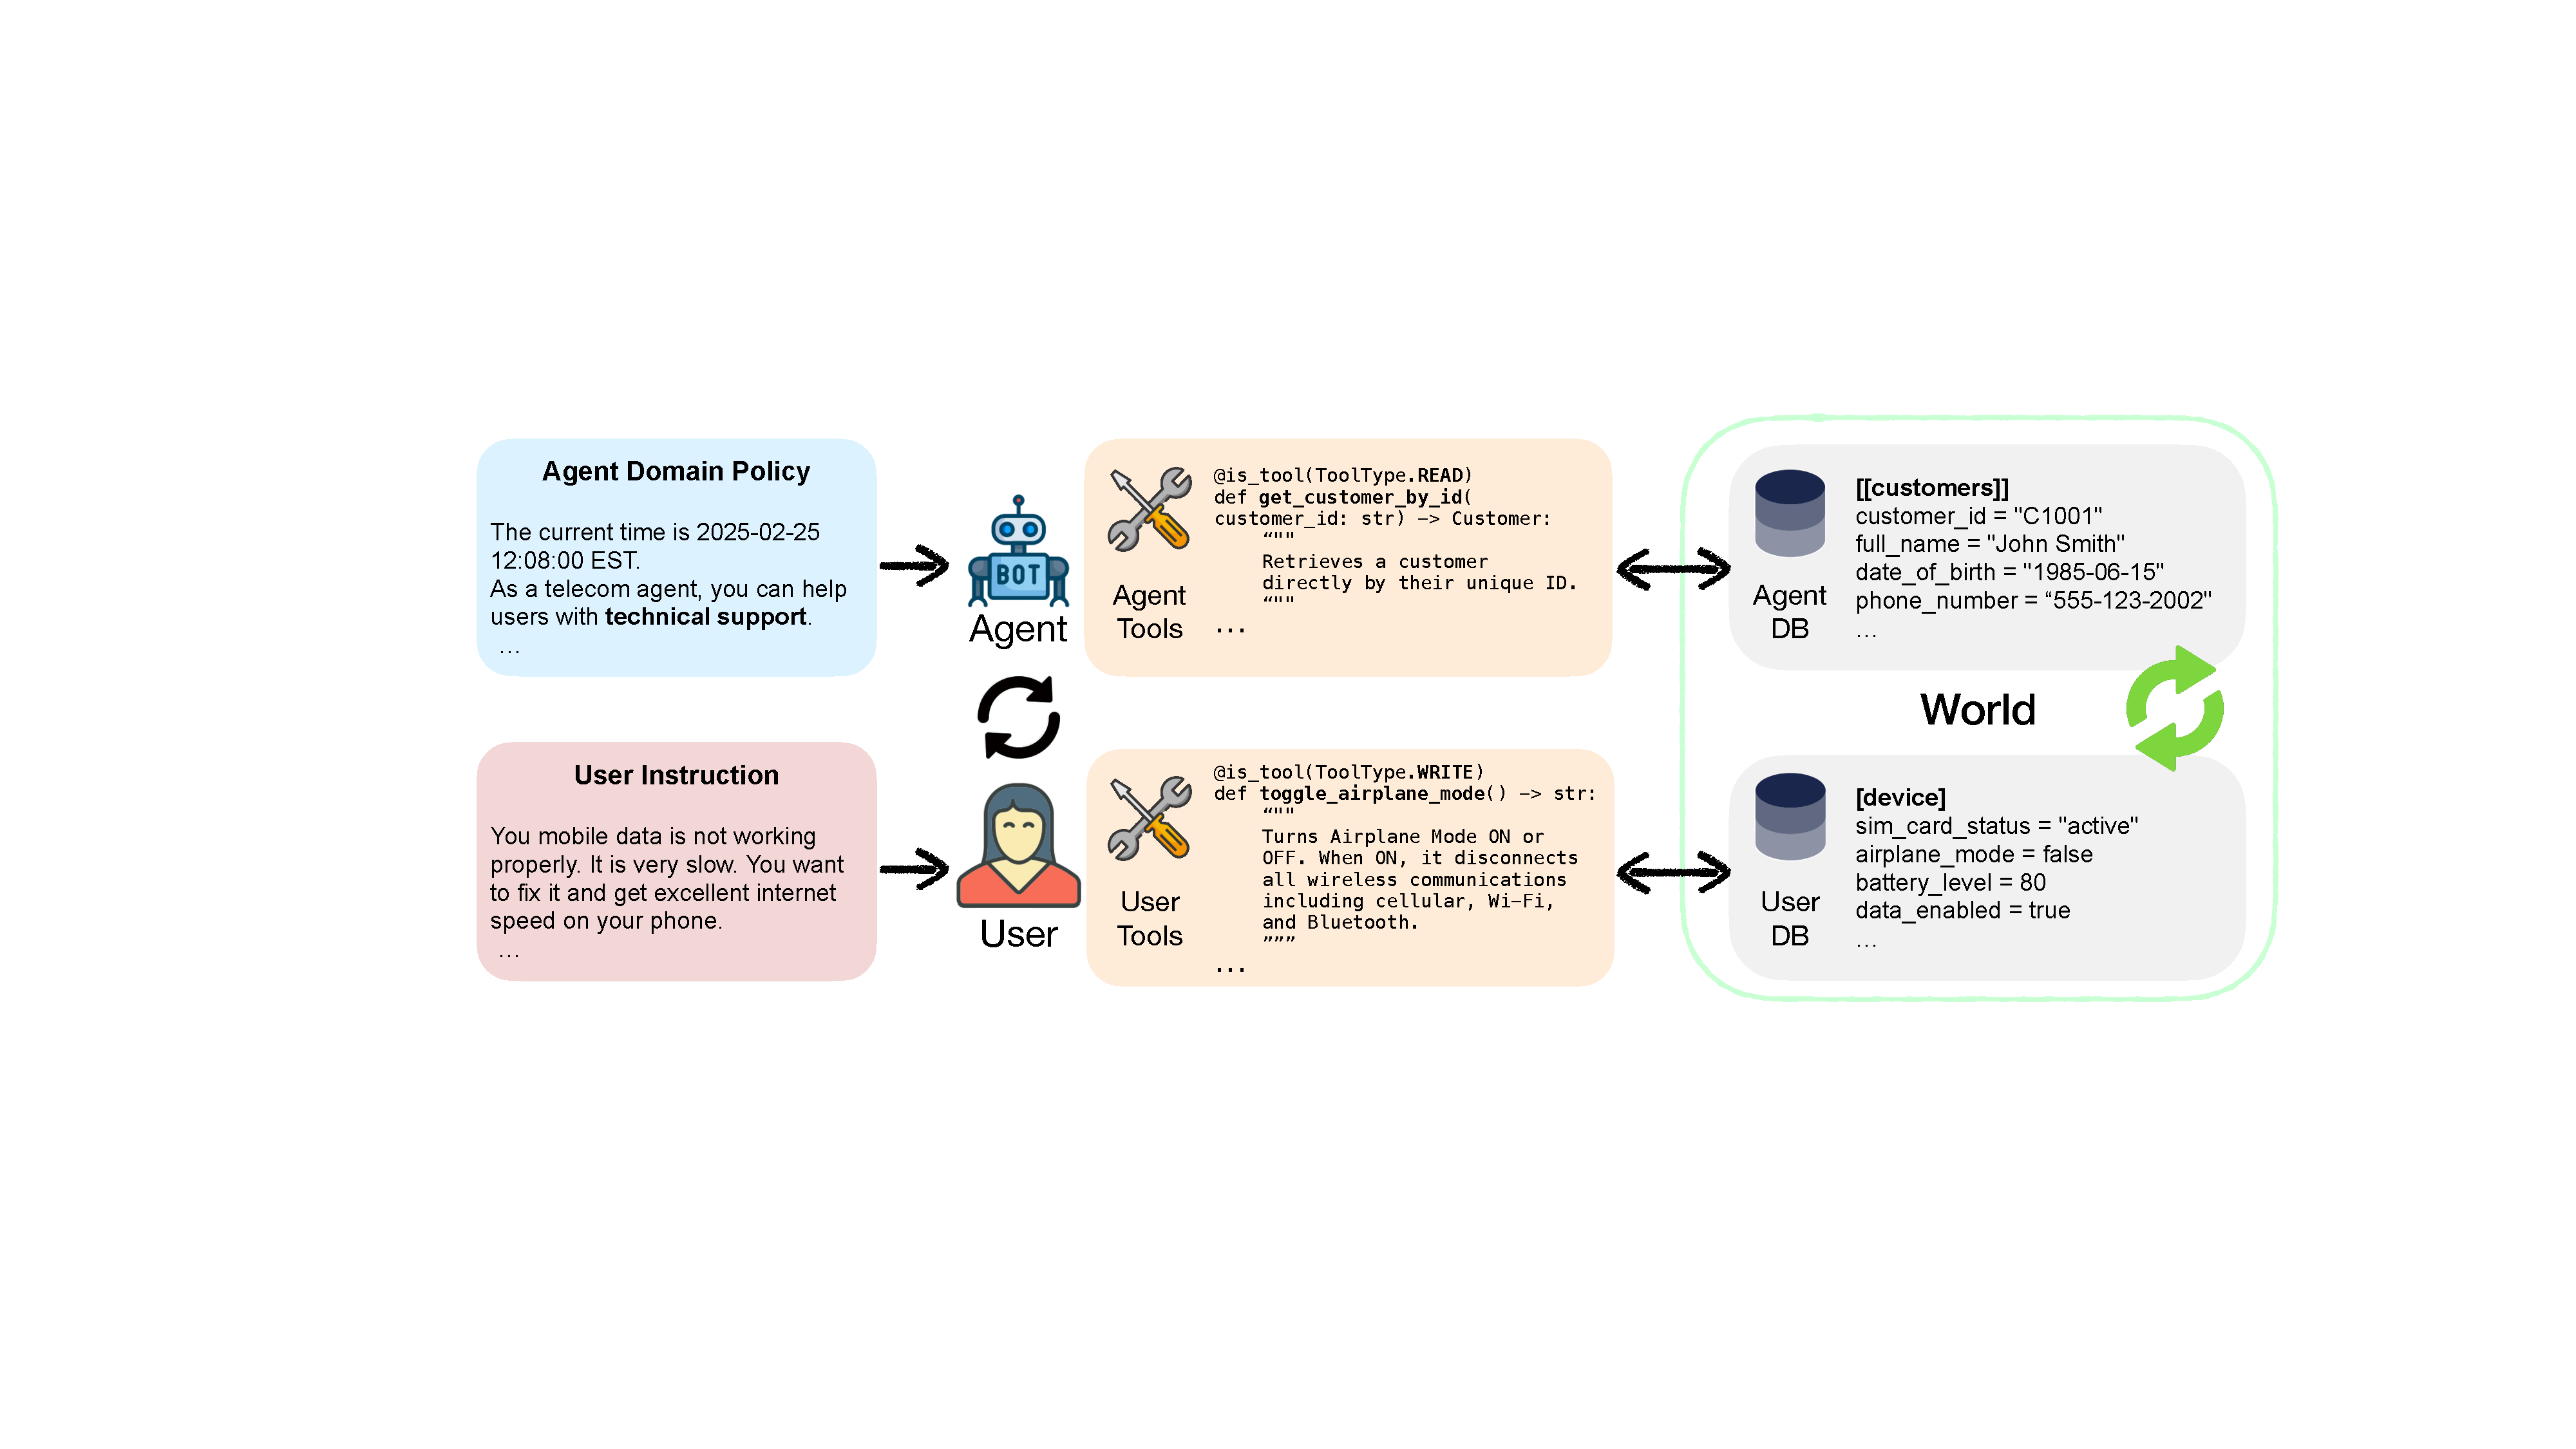
\includegraphics[width=0.99\textwidth,trim=340 330 220 300,clip]{figures/raw/teaser.pdf}
    \vspace{-0.5em}
    \caption{Supporting dual-control environment in \bench. The agent have access to a set of tools that interact with a database, and is tasked with resolving the user's request via Tool-Agent-User (TAU) interactions while adhering to the domain policy. To test real-world scenarios, the user is simulated by another AI agent given a scenario-based instruction and a set of tools that interact with its own database. The simulated user can be regarded as handling an easier version of the TAU interaction in a dual format (Tool-User-Agent), where it only need to follow instructions but does not need to reason about solutions for the task.}
    \label{fig:teaser}
\end{figure}




In such settings, the user's understanding of the agent's environment (including the set of actions the agent can take) is provided through carefully crafted natural language instructions that help ensure a single, solvable path for the constraint satisfaction problem. While this enables easier task specification, the user can only perceive the agent's actions through communication and reason about the environment state solely based on the initial instructions. This is quite different from real-world scenarios like technical customer support, where the user has to actively participate in taking some actions to diagnose and solve problems when asked to do so, such as \textit{restarting their phone} or \textit{turning off airplane mode}.

In order to capture this additional real-world complexity, we introduce \bench with a \textit{dual-control} environment, where (LLM-simulated) users can take actions and call tools in addition to communicating with the agent. The dual-control model provides a few advantages in improving the user simulation, such as selective information hiding, non-verbal manipulation of the environment, and easier specification of the user's task or scenario, especially in cases where the structured format of tools is preferred to unstructured natural language. 

The primary challenge in a dual-control setup lies in granting the user simulator meaningful agency via tools while maintaining the "complexity asymmetry" between the agent and the user simulator -- that is, making sure the user's affordances are limited and the user still requires support from the agent in order to solve issues. While tools for the user simulator could disrupt this balance by increasing its capabilities, we find that carefully designing the tools can help constrain user behavior, leading to more reliable simulations. We achieve this by ensuring user tools yield only human-readable outputs, limiting user planning to reactive tool use based on agent requests, and tightly constraining user behavior through the environment. This results in a controlled testbed for agents that must both think and effectively guide a user to take the right actions. 

Overall, \bench makes four key contributions:

\textbf{Telecom dual-control domain.} We introduce a novel dual-control \telecom domain within \bench, where, unlike previous benchmarks, both the AI agent and the user possess distinct tools to observe, act upon, and verify the state of a shared, dynamic environment. This is formalized using a Decentralized Partially Observable Markov Decision Process (\decpomdp)~\cite{oliehoek2016concise}. This dual-control setup is designed to accurately represent real-world collaborative scenarios and exposes crucial agent coordination and communication challenges absent from evaluations where users have limited agency. Experiments show state-of-the-art LLMs struggle significantly in this domain (e.g., \passone of 34\% for \gptmodelshort \cite{gpt41}, 42\% for \ofourmodelshort \cite{o4mini}, and 49\% for \claudesonnetshort \cite{claude37sonnet} on new tasks).

\textbf{Compositional task generator.} \bench incorporates a programmatic task generator that automatically composes a vast and diverse set of verifiable tasks from a small set of atomic base scenarios (defined by initialization, solution, and assertion functions). This method ensures provable correctness of tasks, provides complete domain coverage, allows for explicit control over task complexity (e.g., by number of solution steps or issue type), and removes the manual effort and potential brittleness associated with hand-crafted task suites.

\textbf{Reliable user simulator.} We enhance the reliability of the user simulation by tightly coupling the user simulator to the environment. User behavior is constrained by the available tools and the observable state of the environment, leading to more predictable and consistent interactions. This approach significantly alleviates the need for complex natural language prompting to guide the user simulator and results in substantially higher reliability (e.g., the \telecom domain's user simulator shows a 16\% error rate with 6\% critical errors, compared to 40\% error rate with 12\% critical errors in the \retail domain from \taubench).

 \textbf{Fine-grained diagnosis of agent failures.} \bench enables a decomposed diagnosis of agent performance by evaluating task success in different modes: (i) a fully autonomous mode (``no-user mode''), where the agent controls all tools, isolating its reasoning capabilities, and (ii) the standard dual-control mode, which introduces communication and coordination requirements. Our findings reveal a substantial performance decrease (around 20\% \passone) when agents must shift from autonomous operation to guiding a user. This clearly distinguishes pure reasoning failures from those arising from communication and decentralized control, pinpointing the latter as a critical bottleneck for current agents.


